\subsection*{Figure S2 -- structures non convergées (avant / dernier cycle)}
Pour chaque candidat non converg\'e (Tableau~S2)~: \`a gauche la g\'eom\'etrie initiale (criblage GFN2-xTB), \`a droite la derni\`ere g\'eom\'etrie tent\'ee par l'optimiseur DFT avant d'atteindre la limite de cycles -- pas un minimum, juste le dernier point de la trajectoire d'optimisation.
\begin{figure}[H]
\centering
\begin{minipage}{0.46\textwidth}
\centering
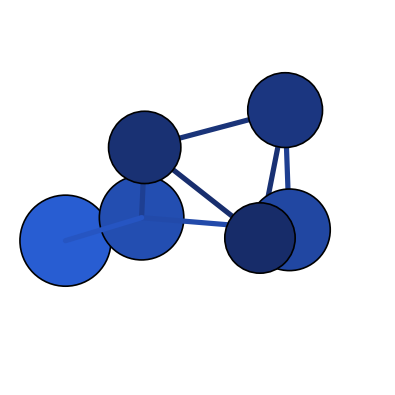
\includegraphics[width=0.8\linewidth]{figs/nonconverged/N6_neutral_neutral_011_initial.png}\\[2pt]
{\small initiale (xTB, N$_6^{0}$)}
\end{minipage}\hfill
\begin{minipage}{0.46\textwidth}
\centering
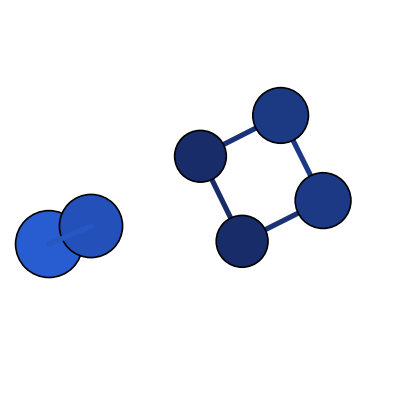
\includegraphics[width=0.8\linewidth]{figs/nonconverged/N6_neutral_neutral_011_last.png}\\[2pt]
{\small dernier cycle DFT (50 cycles)}
\end{minipage}
\end{figure}
\centerline{\small \texttt{N6\_neutral\_neutral\_011} -- en cours de fragmentation, 2$+$4}
\vspace{8pt}
\begin{figure}[H]
\centering
\begin{minipage}{0.46\textwidth}
\centering
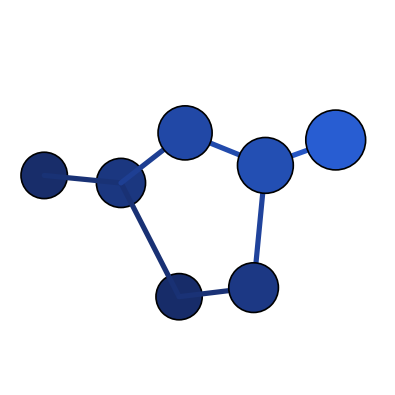
\includegraphics[width=0.8\linewidth]{figs/nonconverged/N7_anion_anion_006_initial.png}\\[2pt]
{\small initiale (xTB, N$_7^{-}$)}
\end{minipage}\hfill
\begin{minipage}{0.46\textwidth}
\centering
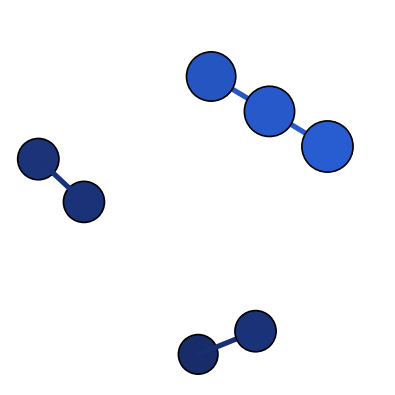
\includegraphics[width=0.8\linewidth]{figs/nonconverged/N7_anion_anion_006_last.png}\\[2pt]
{\small dernier cycle DFT (50 cycles)}
\end{minipage}
\end{figure}
\centerline{\small \texttt{N7\_anion\_anion\_006} -- en cours de fragmentation, 2$+$2$+$3}
\vspace{8pt}
\begin{figure}[H]
\centering
\begin{minipage}{0.46\textwidth}
\centering
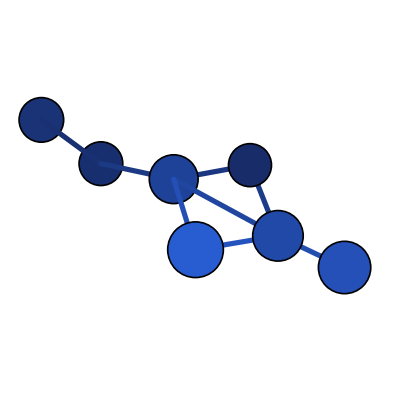
\includegraphics[width=0.8\linewidth]{figs/nonconverged/N7_anion_anion_015_initial.png}\\[2pt]
{\small initiale (xTB, N$_7^{-}$)}
\end{minipage}\hfill
\begin{minipage}{0.46\textwidth}
\centering
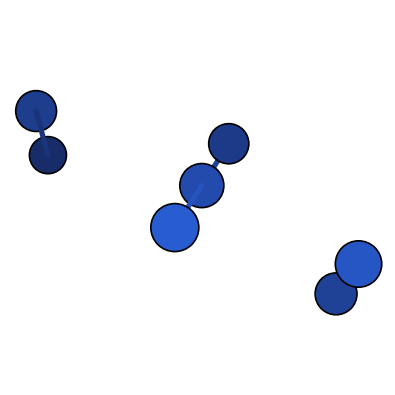
\includegraphics[width=0.8\linewidth]{figs/nonconverged/N7_anion_anion_015_last.png}\\[2pt]
{\small dernier cycle DFT (50 cycles)}
\end{minipage}
\end{figure}
\centerline{\small \texttt{N7\_anion\_anion\_015} -- en cours de fragmentation, 2$+$2$+$3}
\vspace{8pt}
\begin{figure}[H]
\centering
\begin{minipage}{0.46\textwidth}
\centering
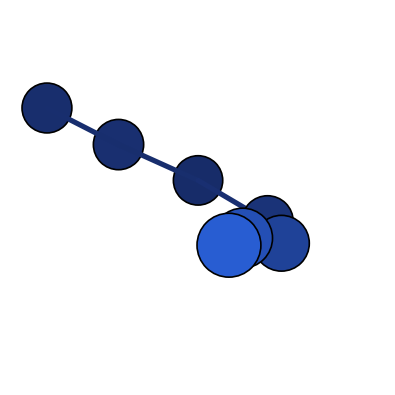
\includegraphics[width=0.8\linewidth]{figs/nonconverged/N7_cation_cation_002_initial.png}\\[2pt]
{\small initiale (xTB, N$_7^{+}$)}
\end{minipage}\hfill
\begin{minipage}{0.46\textwidth}
\centering
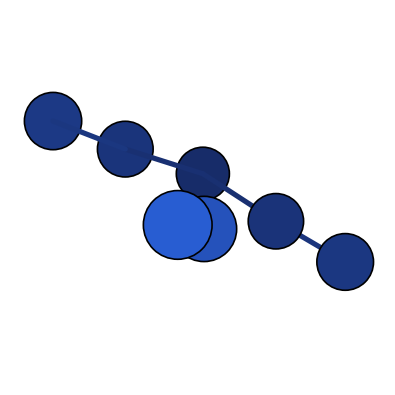
\includegraphics[width=0.8\linewidth]{figs/nonconverged/N7_cation_cation_002_last.png}\\[2pt]
{\small dernier cycle DFT (50 cycles)}
\end{minipage}
\end{figure}
\centerline{\small \texttt{N7\_cation\_cation\_002} -- en cours de fragmentation, 2$+$5}
\vspace{8pt}
\begin{figure}[H]
\centering
\begin{minipage}{0.46\textwidth}
\centering
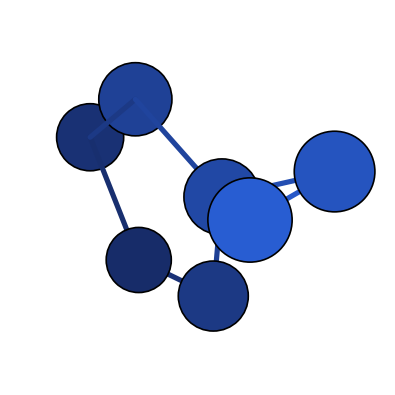
\includegraphics[width=0.8\linewidth]{figs/nonconverged/N7_cation_cation_004_initial.png}\\[2pt]
{\small initiale (xTB, N$_7^{+}$)}
\end{minipage}\hfill
\begin{minipage}{0.46\textwidth}
\centering
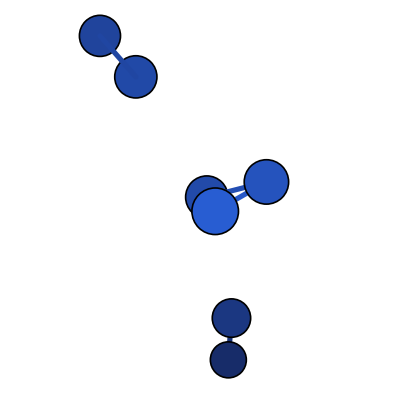
\includegraphics[width=0.8\linewidth]{figs/nonconverged/N7_cation_cation_004_last.png}\\[2pt]
{\small dernier cycle DFT (50 cycles)}
\end{minipage}
\end{figure}
\centerline{\small \texttt{N7\_cation\_cation\_004} -- en cours de fragmentation, 2$+$2$+$3}
\vspace{8pt}
\begin{figure}[H]
\centering
\begin{minipage}{0.46\textwidth}
\centering
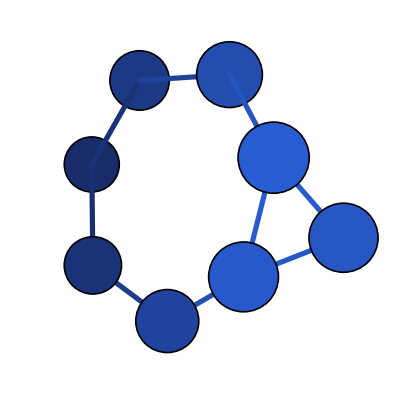
\includegraphics[width=0.8\linewidth]{figs/nonconverged/N8_neutral_neutral_011_initial.png}\\[2pt]
{\small initiale (xTB, N$_8^{0}$)}
\end{minipage}\hfill
\begin{minipage}{0.46\textwidth}
\centering
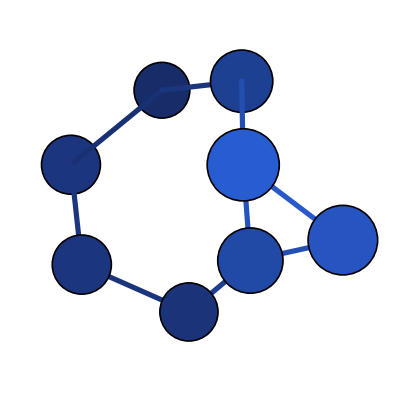
\includegraphics[width=0.8\linewidth]{figs/nonconverged/N8_neutral_neutral_011_last.png}\\[2pt]
{\small dernier cycle DFT (50 cycles)}
\end{minipage}
\end{figure}
\centerline{\small \texttt{N8\_neutral\_neutral\_011} -- cluster unique -- non-convergence num\'erique}
\vspace{8pt}
\begin{figure}[H]
\centering
\begin{minipage}{0.46\textwidth}
\centering
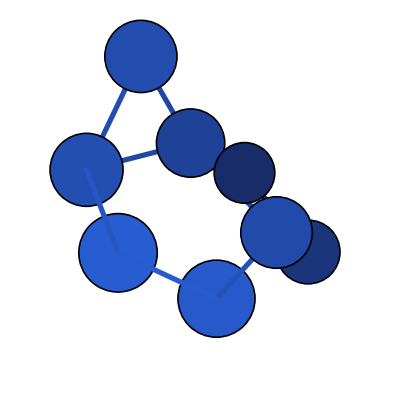
\includegraphics[width=0.8\linewidth]{figs/nonconverged/N8_neutral_neutral_015_initial.png}\\[2pt]
{\small initiale (xTB, N$_8^{0}$)}
\end{minipage}\hfill
\begin{minipage}{0.46\textwidth}
\centering
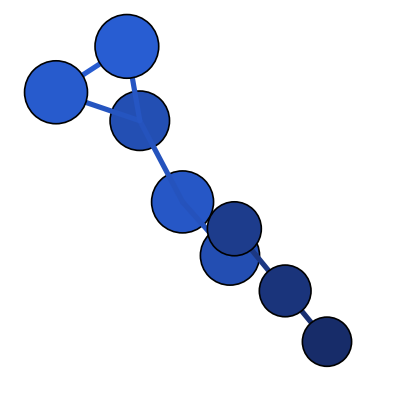
\includegraphics[width=0.8\linewidth]{figs/nonconverged/N8_neutral_neutral_015_last.png}\\[2pt]
{\small dernier cycle DFT (50 cycles)}
\end{minipage}
\end{figure}
\centerline{\small \texttt{N8\_neutral\_neutral\_015} -- cluster unique -- non-convergence num\'erique}
\vspace{8pt}
\begin{figure}[H]
\centering
\begin{minipage}{0.46\textwidth}
\centering
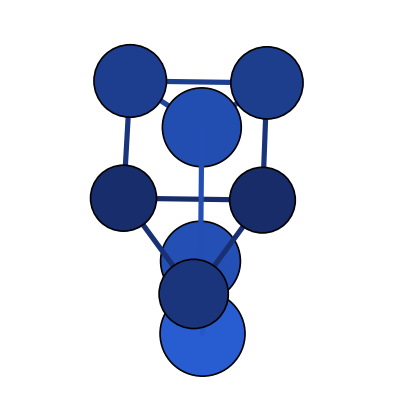
\includegraphics[width=0.8\linewidth]{figs/nonconverged/N8_neutral_neutral_017_initial.png}\\[2pt]
{\small initiale (xTB, N$_8^{0}$)}
\end{minipage}\hfill
\begin{minipage}{0.46\textwidth}
\centering
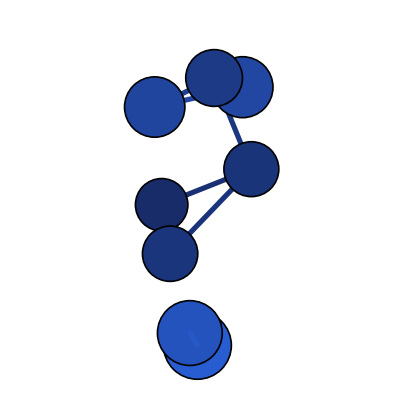
\includegraphics[width=0.8\linewidth]{figs/nonconverged/N8_neutral_neutral_017_last.png}\\[2pt]
{\small dernier cycle DFT (50 cycles)}
\end{minipage}
\end{figure}
\centerline{\small \texttt{N8\_neutral\_neutral\_017} -- en cours de fragmentation, 2$+$6}
\vspace{8pt}
\begin{figure}[H]
\centering
\begin{minipage}{0.46\textwidth}
\centering
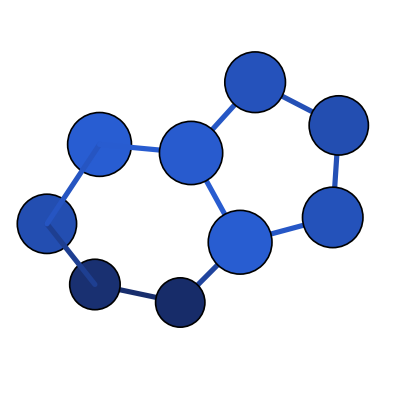
\includegraphics[width=0.8\linewidth]{figs/nonconverged/N9_anion_anion_002_initial.png}\\[2pt]
{\small initiale (xTB, N$_9^{-}$)}
\end{minipage}\hfill
\begin{minipage}{0.46\textwidth}
\centering
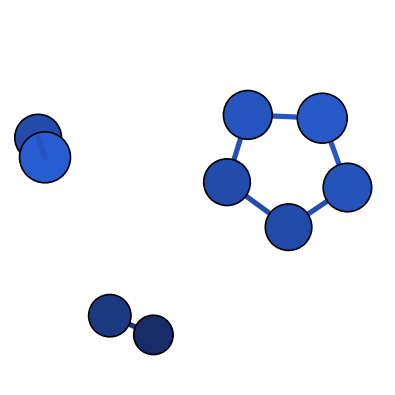
\includegraphics[width=0.8\linewidth]{figs/nonconverged/N9_anion_anion_002_last.png}\\[2pt]
{\small dernier cycle DFT (50 cycles)}
\end{minipage}
\end{figure}
\centerline{\small \texttt{N9\_anion\_anion\_002} -- en cours de fragmentation, 2$+$2$+$5}
\vspace{8pt}
\begin{figure}[H]
\centering
\begin{minipage}{0.46\textwidth}
\centering
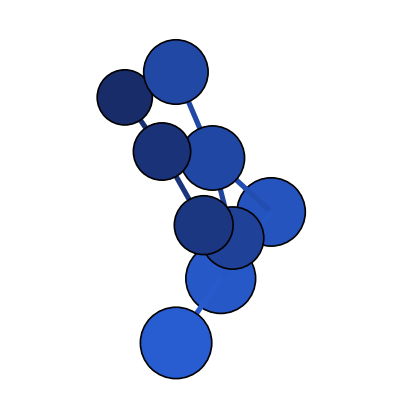
\includegraphics[width=0.8\linewidth]{figs/nonconverged/N9_anion_anion_007_initial.png}\\[2pt]
{\small initiale (xTB, N$_9^{-}$)}
\end{minipage}\hfill
\begin{minipage}{0.46\textwidth}
\centering
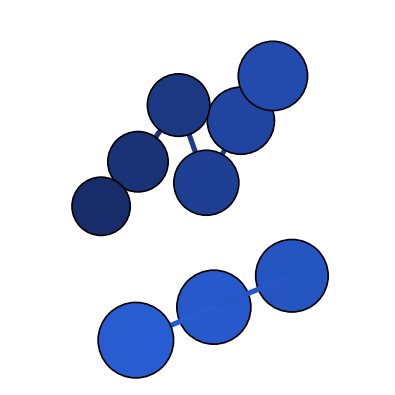
\includegraphics[width=0.8\linewidth]{figs/nonconverged/N9_anion_anion_007_last.png}\\[2pt]
{\small dernier cycle DFT (50 cycles)}
\end{minipage}
\end{figure}
\centerline{\small \texttt{N9\_anion\_anion\_007} -- en cours de fragmentation, 3$+$6}
\vspace{8pt}
\begin{figure}[H]
\centering
\begin{minipage}{0.46\textwidth}
\centering
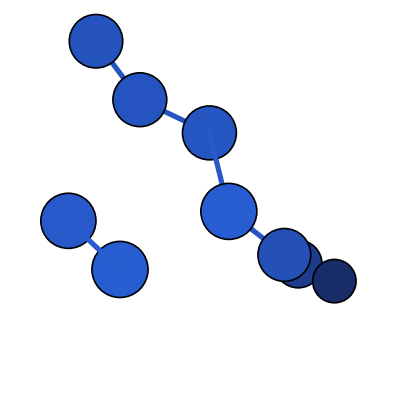
\includegraphics[width=0.8\linewidth]{figs/nonconverged/N9_anion_anion_009_initial.png}\\[2pt]
{\small initiale (xTB, N$_9^{-}$)}
\end{minipage}\hfill
\begin{minipage}{0.46\textwidth}
\centering
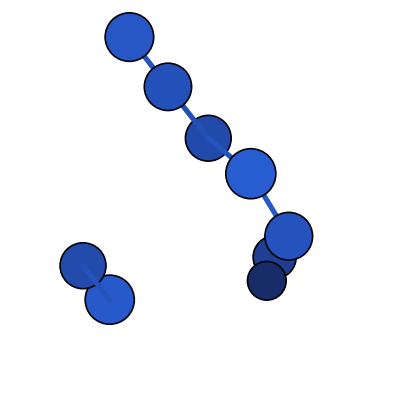
\includegraphics[width=0.8\linewidth]{figs/nonconverged/N9_anion_anion_009_last.png}\\[2pt]
{\small dernier cycle DFT (50 cycles)}
\end{minipage}
\end{figure}
\centerline{\small \texttt{N9\_anion\_anion\_009} -- en cours de fragmentation, 2$+$7}
\vspace{8pt}
\begin{figure}[H]
\centering
\begin{minipage}{0.46\textwidth}
\centering
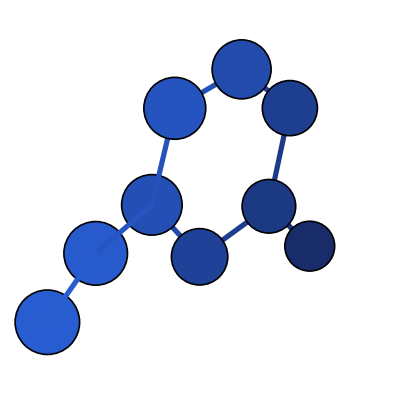
\includegraphics[width=0.8\linewidth]{figs/nonconverged/N9_anion_anion_014_initial.png}\\[2pt]
{\small initiale (xTB, N$_9^{-}$)}
\end{minipage}\hfill
\begin{minipage}{0.46\textwidth}
\centering
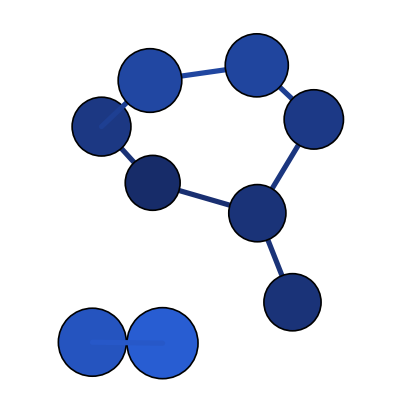
\includegraphics[width=0.8\linewidth]{figs/nonconverged/N9_anion_anion_014_last.png}\\[2pt]
{\small dernier cycle DFT (50 cycles)}
\end{minipage}
\end{figure}
\centerline{\small \texttt{N9\_anion\_anion\_014} -- en cours de fragmentation, 2$+$7}
\vspace{8pt}
\begin{figure}[H]
\centering
\begin{minipage}{0.46\textwidth}
\centering
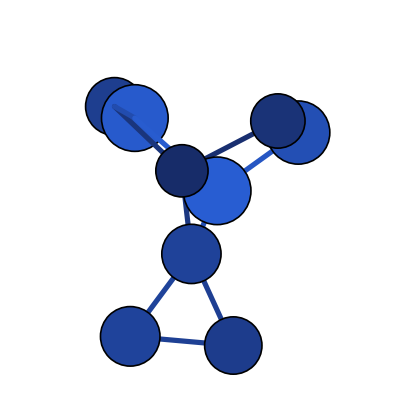
\includegraphics[width=0.8\linewidth]{figs/nonconverged/N9_anion_anion_017_initial.png}\\[2pt]
{\small initiale (xTB, N$_9^{-}$)}
\end{minipage}\hfill
\begin{minipage}{0.46\textwidth}
\centering
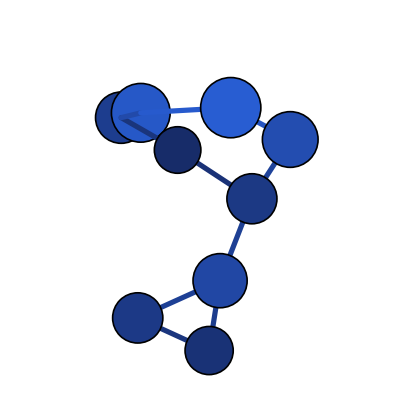
\includegraphics[width=0.8\linewidth]{figs/nonconverged/N9_anion_anion_017_last.png}\\[2pt]
{\small dernier cycle DFT (50 cycles)}
\end{minipage}
\end{figure}
\centerline{\small \texttt{N9\_anion\_anion\_017} -- cluster unique -- non-convergence num\'erique}
\vspace{8pt}
\begin{figure}[H]
\centering
\begin{minipage}{0.46\textwidth}
\centering
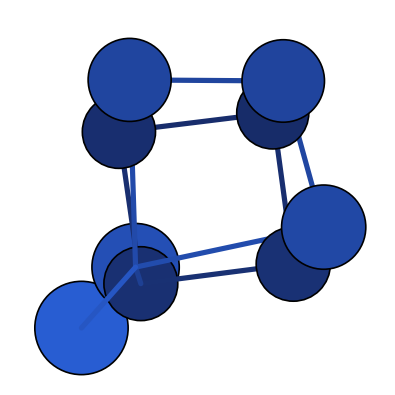
\includegraphics[width=0.8\linewidth]{figs/nonconverged/N9_anion_anion_020_initial.png}\\[2pt]
{\small initiale (xTB, N$_9^{-}$)}
\end{minipage}\hfill
\begin{minipage}{0.46\textwidth}
\centering
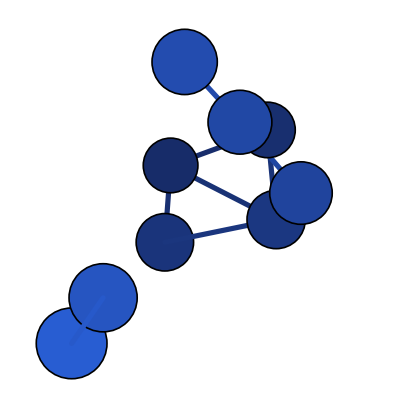
\includegraphics[width=0.8\linewidth]{figs/nonconverged/N9_anion_anion_020_last.png}\\[2pt]
{\small dernier cycle DFT (50 cycles)}
\end{minipage}
\end{figure}
\centerline{\small \texttt{N9\_anion\_anion\_020} -- en cours de fragmentation, 2$+$7}
\vspace{8pt}
\begin{figure}[H]
\centering
\begin{minipage}{0.46\textwidth}
\centering
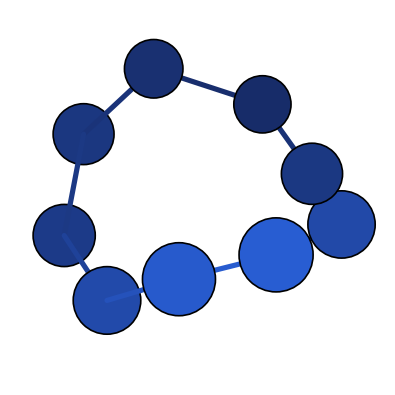
\includegraphics[width=0.8\linewidth]{figs/nonconverged/N9_cation_cation_002_initial.png}\\[2pt]
{\small initiale (xTB, N$_9^{+}$)}
\end{minipage}\hfill
\begin{minipage}{0.46\textwidth}
\centering
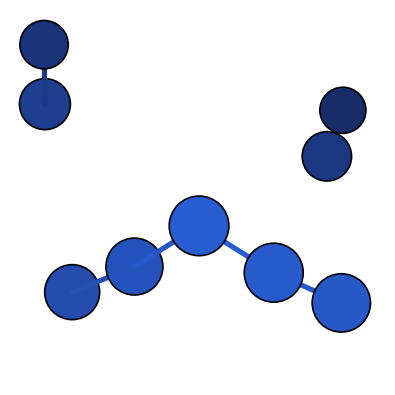
\includegraphics[width=0.8\linewidth]{figs/nonconverged/N9_cation_cation_002_last.png}\\[2pt]
{\small dernier cycle DFT (50 cycles)}
\end{minipage}
\end{figure}
\centerline{\small \texttt{N9\_cation\_cation\_002} -- en cours de fragmentation, 2$+$2$+$5}
\vspace{8pt}
\begin{figure}[H]
\centering
\begin{minipage}{0.46\textwidth}
\centering
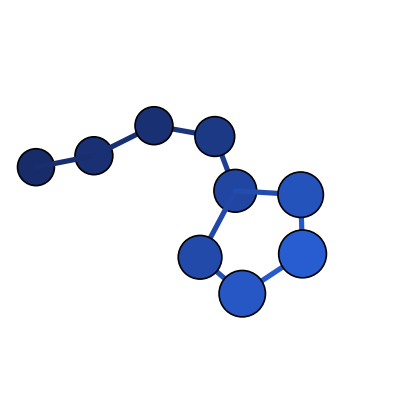
\includegraphics[width=0.8\linewidth]{figs/nonconverged/N9_cation_cation_003_initial.png}\\[2pt]
{\small initiale (xTB, N$_9^{+}$)}
\end{minipage}\hfill
\begin{minipage}{0.46\textwidth}
\centering
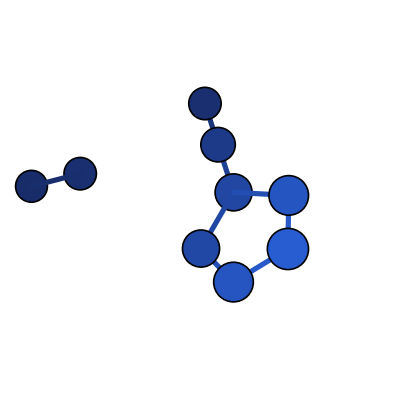
\includegraphics[width=0.8\linewidth]{figs/nonconverged/N9_cation_cation_003_last.png}\\[2pt]
{\small dernier cycle DFT (50 cycles)}
\end{minipage}
\end{figure}
\centerline{\small \texttt{N9\_cation\_cation\_003} -- en cours de fragmentation, 2$+$7}
\vspace{8pt}
\begin{figure}[H]
\centering
\begin{minipage}{0.46\textwidth}
\centering
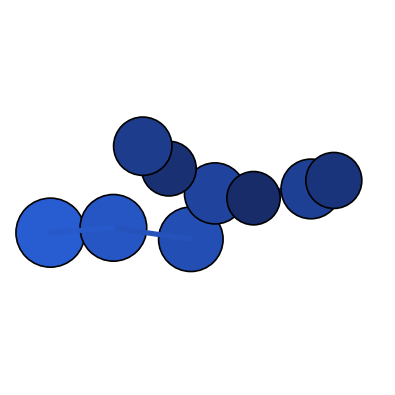
\includegraphics[width=0.8\linewidth]{figs/nonconverged/N9_cation_cation_004_initial.png}\\[2pt]
{\small initiale (xTB, N$_9^{+}$)}
\end{minipage}\hfill
\begin{minipage}{0.46\textwidth}
\centering
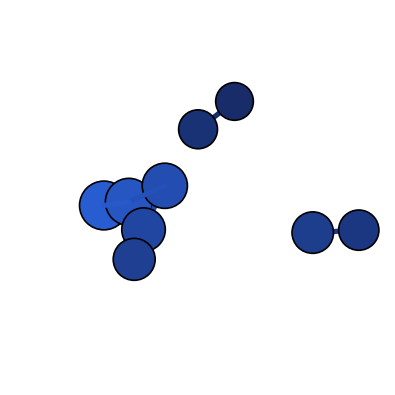
\includegraphics[width=0.8\linewidth]{figs/nonconverged/N9_cation_cation_004_last.png}\\[2pt]
{\small dernier cycle DFT (50 cycles)}
\end{minipage}
\end{figure}
\centerline{\small \texttt{N9\_cation\_cation\_004} -- en cours de fragmentation, 2$+$2$+$5}
\vspace{8pt}
\begin{figure}[H]
\centering
\begin{minipage}{0.46\textwidth}
\centering
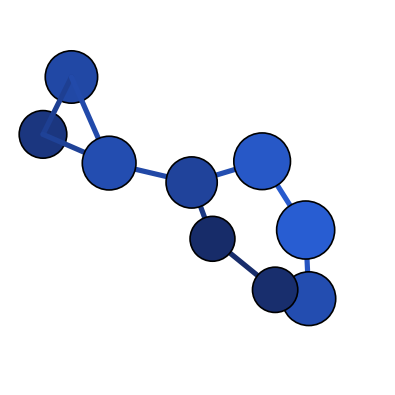
\includegraphics[width=0.8\linewidth]{figs/nonconverged/N9_cation_cation_005_initial.png}\\[2pt]
{\small initiale (xTB, N$_9^{+}$)}
\end{minipage}\hfill
\begin{minipage}{0.46\textwidth}
\centering
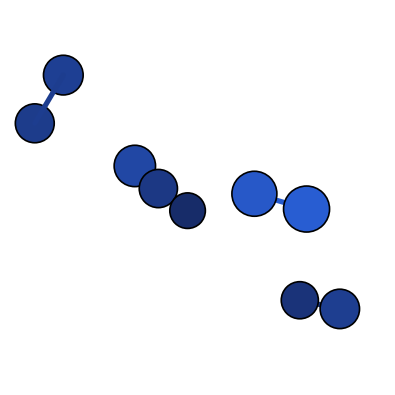
\includegraphics[width=0.8\linewidth]{figs/nonconverged/N9_cation_cation_005_last.png}\\[2pt]
{\small dernier cycle DFT (50 cycles)}
\end{minipage}
\end{figure}
\centerline{\small \texttt{N9\_cation\_cation\_005} -- en cours de fragmentation, 2$+$2$+$2$+$3}
\vspace{8pt}
\begin{figure}[H]
\centering
\begin{minipage}{0.46\textwidth}
\centering
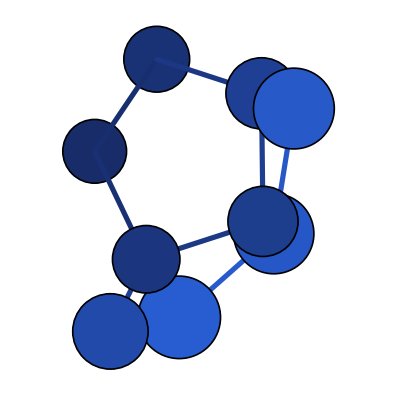
\includegraphics[width=0.8\linewidth]{figs/nonconverged/N9_cation_cation_007_initial.png}\\[2pt]
{\small initiale (xTB, N$_9^{+}$)}
\end{minipage}\hfill
\begin{minipage}{0.46\textwidth}
\centering
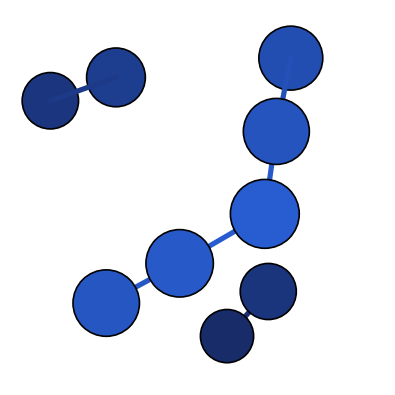
\includegraphics[width=0.8\linewidth]{figs/nonconverged/N9_cation_cation_007_last.png}\\[2pt]
{\small dernier cycle DFT (50 cycles)}
\end{minipage}
\end{figure}
\centerline{\small \texttt{N9\_cation\_cation\_007} -- en cours de fragmentation, 2$+$2$+$5}
\vspace{8pt}
\begin{figure}[H]
\centering
\begin{minipage}{0.46\textwidth}
\centering
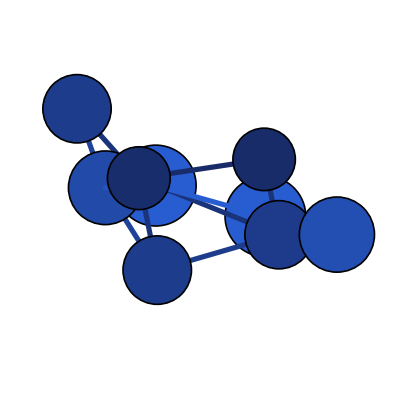
\includegraphics[width=0.8\linewidth]{figs/nonconverged/N9_cation_cation_010_initial.png}\\[2pt]
{\small initiale (xTB, N$_9^{+}$)}
\end{minipage}\hfill
\begin{minipage}{0.46\textwidth}
\centering
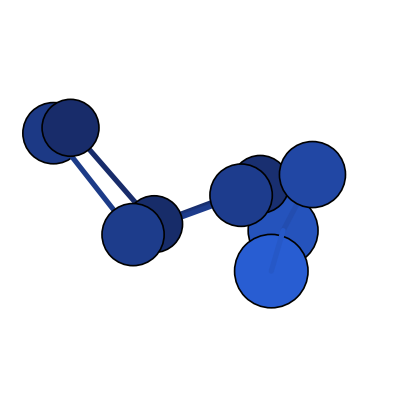
\includegraphics[width=0.8\linewidth]{figs/nonconverged/N9_cation_cation_010_last.png}\\[2pt]
{\small dernier cycle DFT (50 cycles)}
\end{minipage}
\end{figure}
\centerline{\small \texttt{N9\_cation\_cation\_010} -- cluster unique -- non-convergence num\'erique}
\vspace{8pt}
\begin{figure}[H]
\centering
\begin{minipage}{0.46\textwidth}
\centering
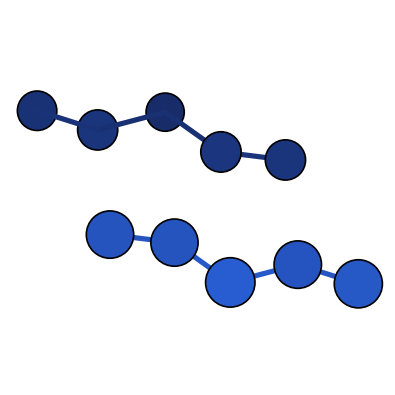
\includegraphics[width=0.8\linewidth]{figs/nonconverged/N10_neutral_neutral_008_initial.png}\\[2pt]
{\small initiale (xTB, N$_10^{0}$)}
\end{minipage}\hfill
\begin{minipage}{0.46\textwidth}
\centering
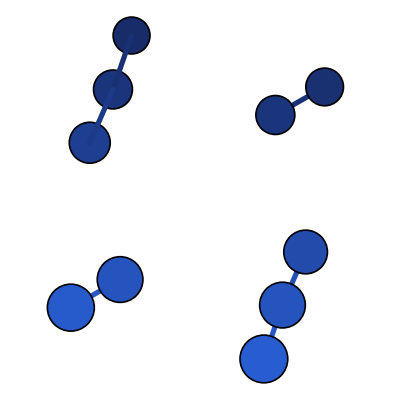
\includegraphics[width=0.8\linewidth]{figs/nonconverged/N10_neutral_neutral_008_last.png}\\[2pt]
{\small dernier cycle DFT (50 cycles)}
\end{minipage}
\end{figure}
\centerline{\small \texttt{N10\_neutral\_neutral\_008} -- en cours de fragmentation, 2$+$2$+$3$+$3}
\vspace{8pt}
\begin{figure}[H]
\centering
\begin{minipage}{0.46\textwidth}
\centering
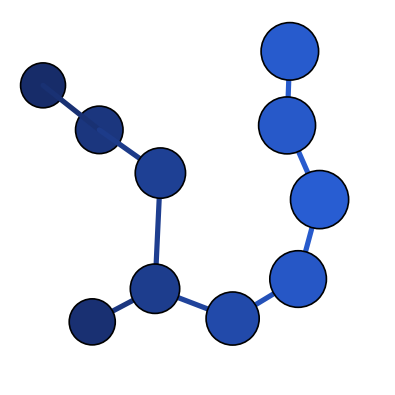
\includegraphics[width=0.8\linewidth]{figs/nonconverged/N10_neutral_neutral_009_initial.png}\\[2pt]
{\small initiale (xTB, N$_10^{0}$)}
\end{minipage}\hfill
\begin{minipage}{0.46\textwidth}
\centering
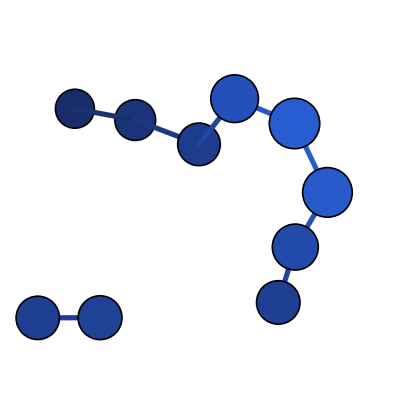
\includegraphics[width=0.8\linewidth]{figs/nonconverged/N10_neutral_neutral_009_last.png}\\[2pt]
{\small dernier cycle DFT (50 cycles)}
\end{minipage}
\end{figure}
\centerline{\small \texttt{N10\_neutral\_neutral\_009} -- en cours de fragmentation, 2$+$8}
\vspace{8pt}
\begin{figure}[H]
\centering
\begin{minipage}{0.46\textwidth}
\centering
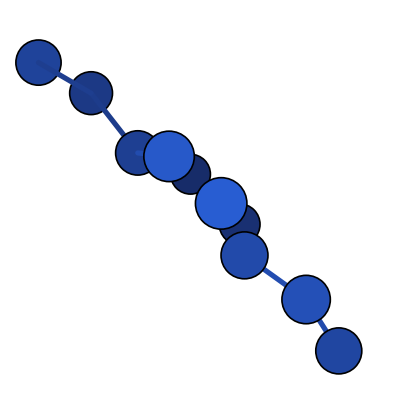
\includegraphics[width=0.8\linewidth]{figs/nonconverged/N10_neutral_neutral_012_initial.png}\\[2pt]
{\small initiale (xTB, N$_10^{0}$)}
\end{minipage}\hfill
\begin{minipage}{0.46\textwidth}
\centering
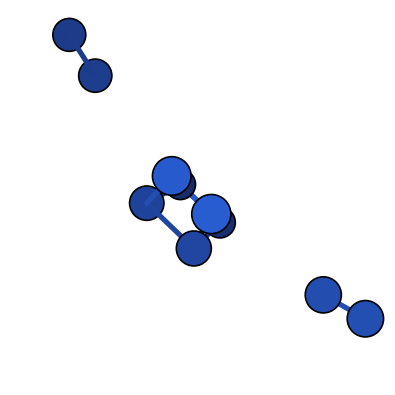
\includegraphics[width=0.8\linewidth]{figs/nonconverged/N10_neutral_neutral_012_last.png}\\[2pt]
{\small dernier cycle DFT (50 cycles)}
\end{minipage}
\end{figure}
\centerline{\small \texttt{N10\_neutral\_neutral\_012} -- en cours de fragmentation, 2$+$2$+$6}
\vspace{8pt}
\begin{figure}[H]
\centering
\begin{minipage}{0.46\textwidth}
\centering
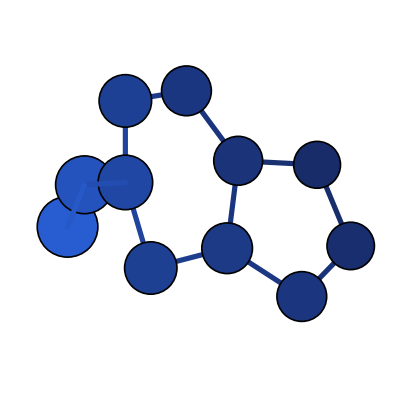
\includegraphics[width=0.8\linewidth]{figs/nonconverged/N11_anion_anion_009_initial.png}\\[2pt]
{\small initiale (xTB, N$_11^{-}$)}
\end{minipage}\hfill
\begin{minipage}{0.46\textwidth}
\centering
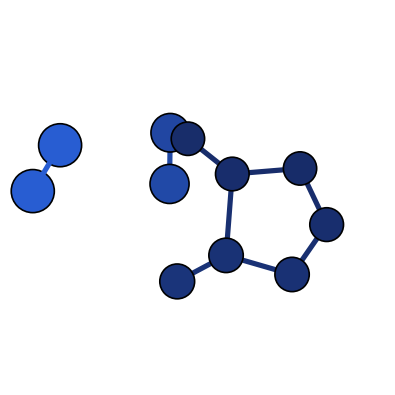
\includegraphics[width=0.8\linewidth]{figs/nonconverged/N11_anion_anion_009_last.png}\\[2pt]
{\small dernier cycle DFT (50 cycles)}
\end{minipage}
\end{figure}
\centerline{\small \texttt{N11\_anion\_anion\_009} -- en cours de fragmentation, 2$+$2$+$7}
\vspace{8pt}
\begin{figure}[H]
\centering
\begin{minipage}{0.46\textwidth}
\centering
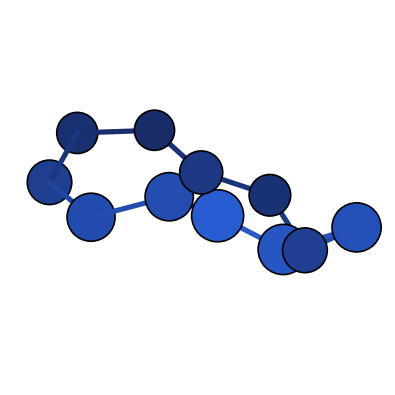
\includegraphics[width=0.8\linewidth]{figs/nonconverged/N11_anion_anion_012_initial.png}\\[2pt]
{\small initiale (xTB, N$_11^{-}$)}
\end{minipage}\hfill
\begin{minipage}{0.46\textwidth}
\centering
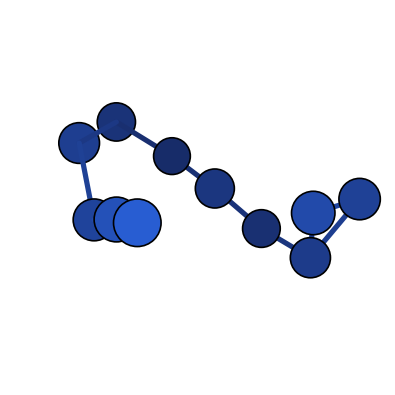
\includegraphics[width=0.8\linewidth]{figs/nonconverged/N11_anion_anion_012_last.png}\\[2pt]
{\small dernier cycle DFT (50 cycles)}
\end{minipage}
\end{figure}
\centerline{\small \texttt{N11\_anion\_anion\_012} -- cluster unique -- non-convergence num\'erique}
\vspace{8pt}
\begin{figure}[H]
\centering
\begin{minipage}{0.46\textwidth}
\centering
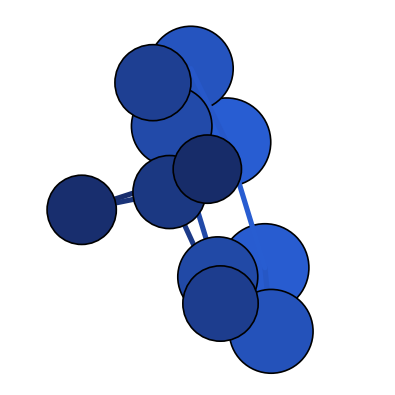
\includegraphics[width=0.8\linewidth]{figs/nonconverged/N11_anion_anion_014_initial.png}\\[2pt]
{\small initiale (xTB, N$_11^{-}$)}
\end{minipage}\hfill
\begin{minipage}{0.46\textwidth}
\centering
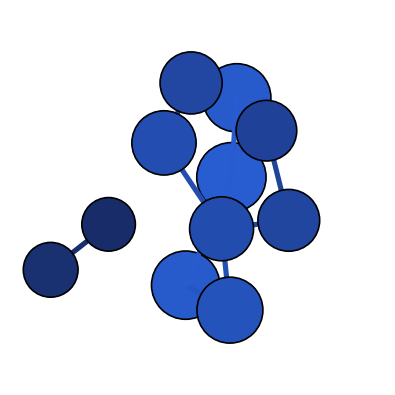
\includegraphics[width=0.8\linewidth]{figs/nonconverged/N11_anion_anion_014_last.png}\\[2pt]
{\small dernier cycle DFT (50 cycles)}
\end{minipage}
\end{figure}
\centerline{\small \texttt{N11\_anion\_anion\_014} -- en cours de fragmentation, 2$+$9}
\vspace{8pt}
\begin{figure}[H]
\centering
\begin{minipage}{0.46\textwidth}
\centering
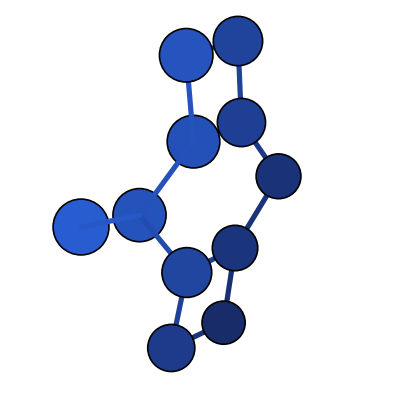
\includegraphics[width=0.8\linewidth]{figs/nonconverged/N11_anion_anion_015_initial.png}\\[2pt]
{\small initiale (xTB, N$_11^{-}$)}
\end{minipage}\hfill
\begin{minipage}{0.46\textwidth}
\centering
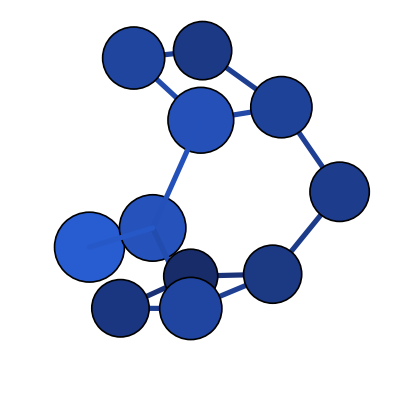
\includegraphics[width=0.8\linewidth]{figs/nonconverged/N11_anion_anion_015_last.png}\\[2pt]
{\small dernier cycle DFT (50 cycles)}
\end{minipage}
\end{figure}
\centerline{\small \texttt{N11\_anion\_anion\_015} -- cluster unique -- non-convergence num\'erique}
\vspace{8pt}
\begin{figure}[H]
\centering
\begin{minipage}{0.46\textwidth}
\centering
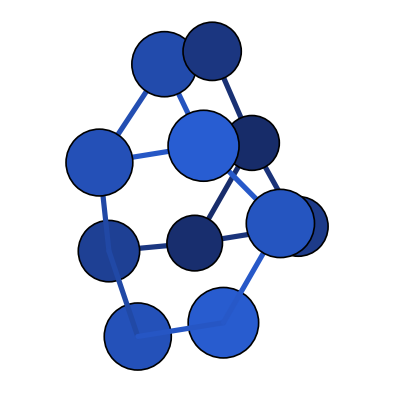
\includegraphics[width=0.8\linewidth]{figs/nonconverged/N11_anion_anion_016_initial.png}\\[2pt]
{\small initiale (xTB, N$_11^{-}$)}
\end{minipage}\hfill
\begin{minipage}{0.46\textwidth}
\centering
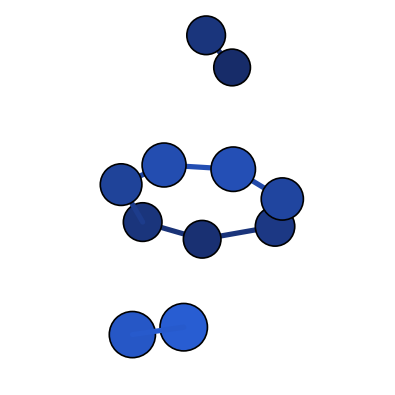
\includegraphics[width=0.8\linewidth]{figs/nonconverged/N11_anion_anion_016_last.png}\\[2pt]
{\small dernier cycle DFT (50 cycles)}
\end{minipage}
\end{figure}
\centerline{\small \texttt{N11\_anion\_anion\_016} -- en cours de fragmentation, 2$+$2$+$7}
\vspace{8pt}
\begin{figure}[H]
\centering
\begin{minipage}{0.46\textwidth}
\centering
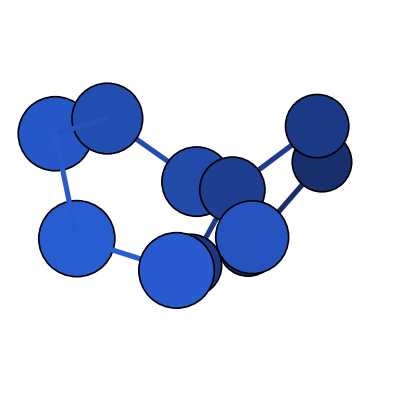
\includegraphics[width=0.8\linewidth]{figs/nonconverged/N11_cation_cation_003_initial.png}\\[2pt]
{\small initiale (xTB, N$_11^{+}$)}
\end{minipage}\hfill
\begin{minipage}{0.46\textwidth}
\centering
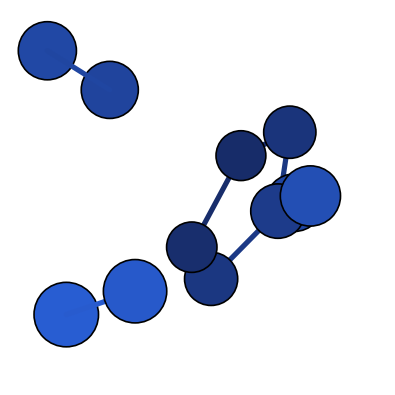
\includegraphics[width=0.8\linewidth]{figs/nonconverged/N11_cation_cation_003_last.png}\\[2pt]
{\small dernier cycle DFT (50 cycles)}
\end{minipage}
\end{figure}
\centerline{\small \texttt{N11\_cation\_cation\_003} -- en cours de fragmentation, 2$+$2$+$7}
\vspace{8pt}
\begin{figure}[H]
\centering
\begin{minipage}{0.46\textwidth}
\centering
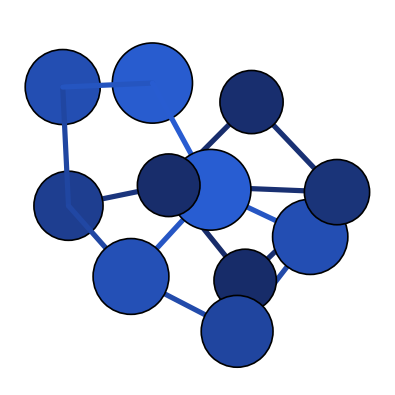
\includegraphics[width=0.8\linewidth]{figs/nonconverged/N11_cation_cation_008_initial.png}\\[2pt]
{\small initiale (xTB, N$_11^{+}$)}
\end{minipage}\hfill
\begin{minipage}{0.46\textwidth}
\centering
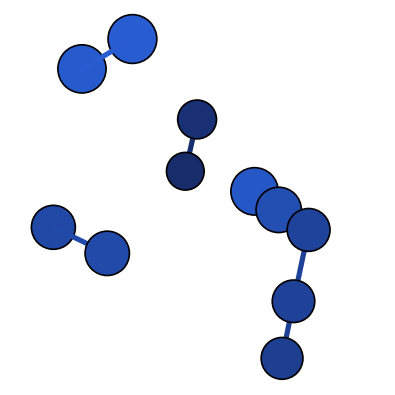
\includegraphics[width=0.8\linewidth]{figs/nonconverged/N11_cation_cation_008_last.png}\\[2pt]
{\small dernier cycle DFT (50 cycles)}
\end{minipage}
\end{figure}
\centerline{\small \texttt{N11\_cation\_cation\_008} -- en cours de fragmentation, 2$+$2$+$2$+$5}
\vspace{8pt}
\begin{figure}[H]
\centering
\begin{minipage}{0.46\textwidth}
\centering
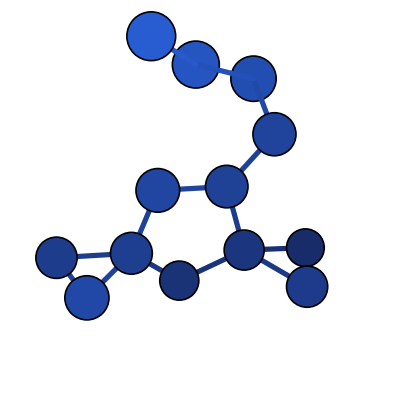
\includegraphics[width=0.8\linewidth]{figs/nonconverged/N13_anion_anion_002_initial.png}\\[2pt]
{\small initiale (xTB, N$_13^{-}$)}
\end{minipage}\hfill
\begin{minipage}{0.46\textwidth}
\centering
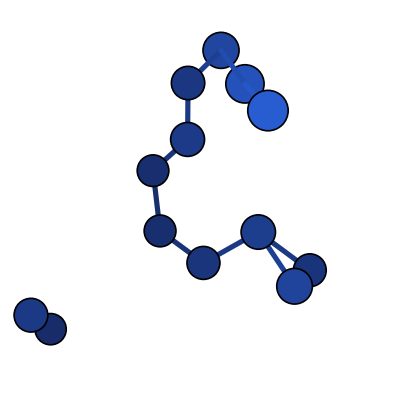
\includegraphics[width=0.8\linewidth]{figs/nonconverged/N13_anion_anion_002_last.png}\\[2pt]
{\small dernier cycle DFT (50 cycles)}
\end{minipage}
\end{figure}
\centerline{\small \texttt{N13\_anion\_anion\_002} -- en cours de fragmentation, 2$+$11}
\vspace{8pt}
\begin{figure}[H]
\centering
\begin{minipage}{0.46\textwidth}
\centering
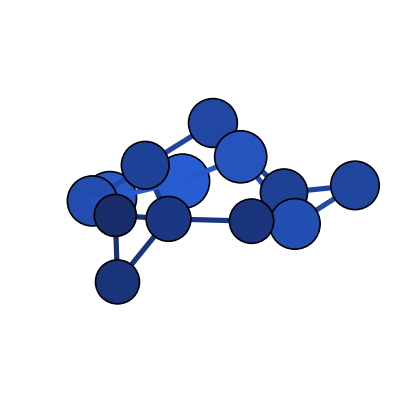
\includegraphics[width=0.8\linewidth]{figs/nonconverged/N13_anion_anion_003_initial.png}\\[2pt]
{\small initiale (xTB, N$_13^{-}$)}
\end{minipage}\hfill
\begin{minipage}{0.46\textwidth}
\centering
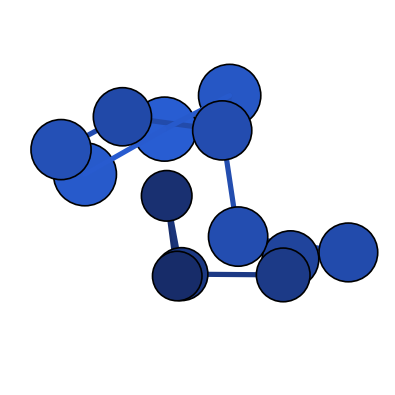
\includegraphics[width=0.8\linewidth]{figs/nonconverged/N13_anion_anion_003_last.png}\\[2pt]
{\small dernier cycle DFT (50 cycles)}
\end{minipage}
\end{figure}
\centerline{\small \texttt{N13\_anion\_anion\_003} -- cluster unique -- non-convergence num\'erique}
\vspace{8pt}
\begin{figure}[H]
\centering
\begin{minipage}{0.46\textwidth}
\centering
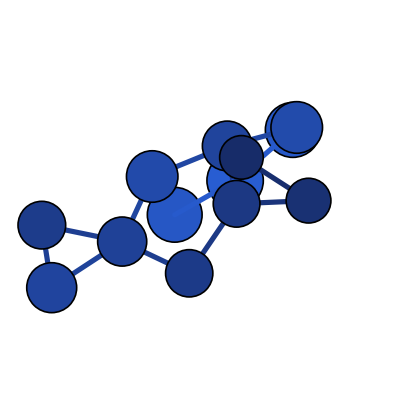
\includegraphics[width=0.8\linewidth]{figs/nonconverged/N13_anion_anion_004_initial.png}\\[2pt]
{\small initiale (xTB, N$_13^{-}$)}
\end{minipage}\hfill
\begin{minipage}{0.46\textwidth}
\centering
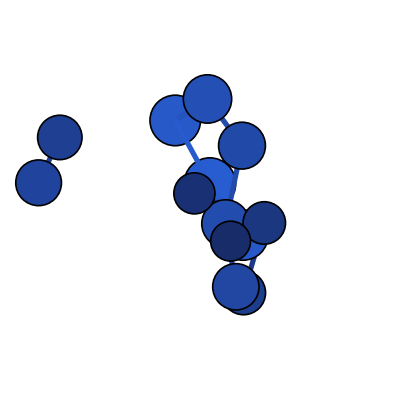
\includegraphics[width=0.8\linewidth]{figs/nonconverged/N13_anion_anion_004_last.png}\\[2pt]
{\small dernier cycle DFT (50 cycles)}
\end{minipage}
\end{figure}
\centerline{\small \texttt{N13\_anion\_anion\_004} -- en cours de fragmentation, 2$+$11}
\vspace{8pt}
\begin{figure}[H]
\centering
\begin{minipage}{0.46\textwidth}
\centering
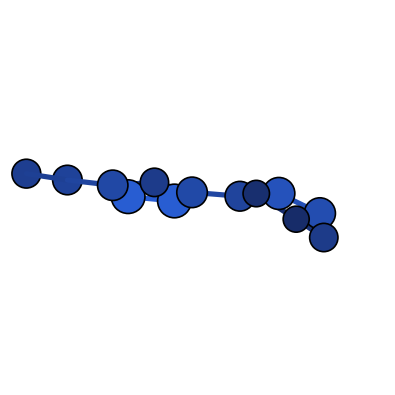
\includegraphics[width=0.8\linewidth]{figs/nonconverged/N13_cation_cation_002_initial.png}\\[2pt]
{\small initiale (xTB, N$_13^{+}$)}
\end{minipage}\hfill
\begin{minipage}{0.46\textwidth}
\centering
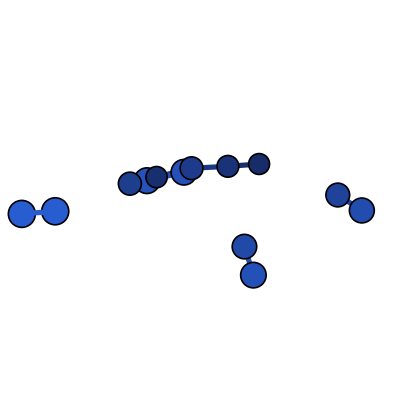
\includegraphics[width=0.8\linewidth]{figs/nonconverged/N13_cation_cation_002_last.png}\\[2pt]
{\small dernier cycle DFT (50 cycles)}
\end{minipage}
\end{figure}
\centerline{\small \texttt{N13\_cation\_cation\_002} -- en cours de fragmentation, 2$+$2$+$2$+$7}
\vspace{8pt}
\begin{figure}[H]
\centering
\begin{minipage}{0.46\textwidth}
\centering
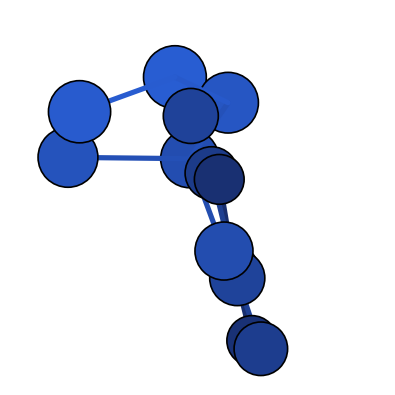
\includegraphics[width=0.8\linewidth]{figs/nonconverged/N13_cation_cation_003_initial.png}\\[2pt]
{\small initiale (xTB, N$_13^{+}$)}
\end{minipage}\hfill
\begin{minipage}{0.46\textwidth}
\centering
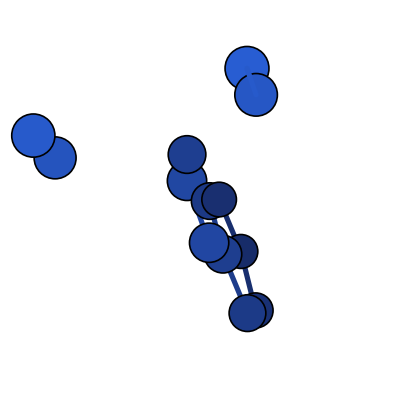
\includegraphics[width=0.8\linewidth]{figs/nonconverged/N13_cation_cation_003_last.png}\\[2pt]
{\small dernier cycle DFT (50 cycles)}
\end{minipage}
\end{figure}
\centerline{\small \texttt{N13\_cation\_cation\_003} -- en cours de fragmentation, 2$+$2$+$9}
\vspace{8pt}
\bigskip\noindent\textit{L\'egende g\'en\'erale, Figure~S2~:} sph\`eres bleues reli\'ees par des b\^atonnets = atomes N et liaisons N--N (mod\`ele boules-b\^atonnets, rendu depuis les coordonn\'ees cart\'esiennes .xyz) ; paires group\'ees par candidat, g\'eom\'etrie initiale GFN2-xTB \`a gauche et derni\`ere g\'eom\'etrie de la trajectoire d'optimisation DFT (non converg\'ee) \`a droite, pour les 35 candidats non converg\'es (Tableau~S2).